\addcontentsline{toc}{chapter}{Chapitre 2 : Mise en Ouevre de Projey } 
\section{Introduction}
Dans ce chapitre, nous allons commencer par illustrer le sprint 0 de notre projet.
Ensuite nous aurons recours aux explications des différents termes caractérisant notre projet.\\
Par la suite, nous allons définir les besoins spécifiques de notre projet, ainsi que le Backlog Produit permettant de déterminer les fonctionnalités de base de ce projet selon la difficulté et la priorité. En addition, nous allons présenter les outils utilisés, illustrer l’architecture et établir le diagramme de cas d’utilisation.

\section{Spécification des besoins}
Les besoins fonctionnels et non fonctionnels feront le but de cette partie ce qui nous permettra de concevoir les objectifs de InnoThink.

La phase d’analyse est primordiale dans le cycle de développement d’une application
afin de bien répartir le projet sur des sprints comme l’indique la méthodologie SCRUM.
\subsection{Identification des acteurs}
\begin{comment}
\begin{table}[h!]
    \centering
    \begin{tabular}{|l|l|l|}
        \hline
        \textbf{Acteur} & \textbf{Type Acteur} & \textbf{Description} \\
        \hline
        \multirow{4}{*}{Utilisateur} & Acteur Principal (physique) & Authentifier, Connecter au VPN, Joindre un réseau, Créer un réseau \\
        \cline{2-3}
        & & Modifier un réseau, Supprimer un réseau, Supprimer un utilisateur, Modifier un utilisateur, Créer un utilisateur \\ 
        \hline
        \multirow{5}{*}{Serveur-Web} & Acteur Secondaire (moral) & Enregistrer chaque modification d’un utilisateur dans la base de données \\
        \cline{2-3}
        & & Enregistrer chaque modification d’un réseau dans la base de données \\
        \cline{2-3}
        & & Joindre l’utilisateur dans un réseau \\
        \cline{2-3}
        & & Créer le nouveau réseau de l’utilisateur \\
        \cline{2-3}
        & & Rassembler chaque utilisateur dans un réseau privé \\
        \hline
        \multirow{3}{*}{Serveur-VPN} & Acteur Secondaire (moral) & Transmet le trafic au utilisateur \\
        \cline{2-3}
        & & Donne une adresse publique à l’utilisateur \\
        \cline{2-3}
        & & Donne une adresse privée à l’utilisateur \\
        \hline
    \end{tabular}
    \caption{Description des acteurs}
    \label{tab:acteurs}
\end{table}
\end{comment}









\textbf{L’admin: }L’acteur principal qui a le rôle le plus important de gèrer l’administration de la plateforme.


\textbf{Le visiteur:} L’acteur secondaire qu’il va découvrir les cours de la plateforme sans s’authentifier.


\\ \textbf{Collaborateur:} L’acteur qui va utiliser les services de la plateforme.


\\ \textbf{Formateur:} L'acteur celui qui va déposer un support de cours


\subsection{Les besoins fonctionnels}
Les exigences fonctionnelles de notre solution sont classées selon les acteurs
impliqués.ainsi que l'assignation des rôles à chaque utilisateur.


\textbf{Gestion des accès à la plateforme :} Cela inclut la création, la modification, la suppression des comptes
\textbf{Gestion des exercies :}Ce module inclut le dépôt des exercies , leur modification et leur suppression.

 
\textbf{Gestion des avis:}  Cela inclut l'ajout, la modification et la suppression des avis.   

\vspace{9mm}

\textbf{Gestion des utilisateur :} Cela inclu , la modifications et la suppression des données des utilisateurs ( étudiant ou professeur ) 




\subsection{Les besoins non fonctionnels}

Les exigences non fonctionnelles définissent le comportement et la performance que le produit doit présenter.
\begin{itemize}
\item \textbf{La performance :} Il est essentiel que la plateforme soit rapide et réactive, garantissant une expérience utilisateur fluide même lorsqu'il y a un grand nombre d'utilisateurs en même temps.

\item \textbf{La sécurité: }La sécurité des donnés des utilisateurs est essentielle ou il doit utiliser des protocoles de cryptage afin de préserver les informations confidentielles telles que les identifiants de connexion et les informations d’authentification

\item \textbf{La disponibilité :}Il est essentiel que la plateforme soit accessible tous les 24 heureset les 7 jours, avec un temps d'arrêt minimal afin de garantir l'accès au cours et aux ressources à tout moment.

\item \textbf{La facilité:} La plateforme devrait être facile à utiliser, avec une interface intuitive et des instructions claires pour faciliter la navigation et l'utilisation des cours et des ressources disponibles.

\item \textbf{Accessibilité :}  La plateforme doit être accessible à tous les utilisateurs, y compris ceux qui ayant des besoins spécifiques en matière d'accessibilité.
\end{itemize}

\newpage
\subsection{Backlog produit}

	\begin{table}[H] % Changed to table for single-column layout
	    \centering
	    \begin{tabular}{|p{3cm}|p{1.5cm}|p{7cm}|p{1.3cm}|}
	        \hline
	        Spirnt & ID User Story & User Story & Priorité \\
	        \hline
	        Gestion d'accès de la plateforme & 1.1 & En tant que visiteur je veux m'inscrire & 3 \\ \hline
        & 1.2 &  En tant que étudiant je veux m’authentifier & 4 \\ \hline 
        & 1.2 &  En tant que professeur je veux m'authentifer  mon compte & 4 \\ \hline 
        & 1.2 &  En tant que admin je veux m'authentifier & 4 \\ \hline 
		









        Gestion des exercices 
        & 2.1 &  En tant que visiteur je veux consulter les exercies & 3 \\ \hline
        & 2.1 &  En tant que étudiant je veux chercher un exercises & 3 \\ \hline
        & 2.1 &  En tant que étudiant je veux m’inscrire à un series des exercies & 3 \\ \hline
        & 2.1 &  En tant que étudiant je veux consulter le progrès des exercies & 3 \\ \hline
        & 2.1 &  En tant que professeur je veux déposer un ou des exercies & 3 \\ \hline
        & 2.1 & En tant que professeur je veux supprimer un exercies & 3 \\ \hline
        & 2.1 & En tant que administrateur je veux consulter un exercies & 3 \\ \hline
        & 2.1 & En tant que administrateur je veux déposer un exercies & 3 \\ \hline
        & 2.1 & En tant que administrateur je veux supprimer un exercies & 3 \\ \hline












        Gestion des avis & 3.1 &  En tant que visiteur je veux consulter les avis & 9 \\ \hline
        & 3.2 &  En tant que étudiant je veux consulter les avis & 10 \\ \hline
        & 3.3 &  En tant que étudiant je veux donner un avis & 10 \\ \hline
        & 3.4 & En tant que professeur je veux consulter les avis & 10 \\ \hline	
        & 3.5 & En tant que professeur je veux donner un avis & 10 \\ \hline
        & 3.5 & En tant que admin je veux consulter les avis & 10 \\ \hline
        & 3.5 & En tant que admin je veux supprimer un avis & 10 \\ \hline










     
    \end{tabular}
    \caption \centering{Backlog produit globale}
    \label{tab:my_label}
	\end{table}











	\begin{table}[H] % Changed to table for single-column layout
	    \centering
	    \begin{tabular}{|p{3cm}|p{1.5cm}|p{7cm}|p{1.3cm}|}
	        \hline
	        Spirnt & ID User Story & User Story & Priorité \\
	        \hline
            Gestion des utilisateurs  & 4.1 & en tant que administrateur je veux consulter les utilisateurs de la platform & 9 \\ \hline
        & 4.2 & en tant que administrateur je veux créer un nouveau utilisateur & 10 \\ \hline
        & 4.3 & en tant que administrateur je veux modifier les utilisateurs & \\ \hline
        & 4.3 & en tant que administrateur je veux supprimer des utilisateurs & \\ \hline
    \end{tabular}
    \caption \centering{Backlog produit globale}
    \label{tab:my_label}
	\end{table}








\subsection{Diagramme de cas d'utilisation globale}
\\
Chaque interaction entre les utilisateurs et le système est définie comme un cas d'utilisation.
Chaque cas d'utilisation représente une fonctionnalité offerte aux utilisateurs pour atteindre un résultat spécifique. Le diagramme de cas d'utilisation décrit donc cette interaction en identifiant les besoins de l'utilisateur et toutes les actions que le système doit effectuer pour répondre à ces besoins.

%DIAGRAMME DE CAS D UTILISATION
  \begin{figure}[h]%
    \center%
    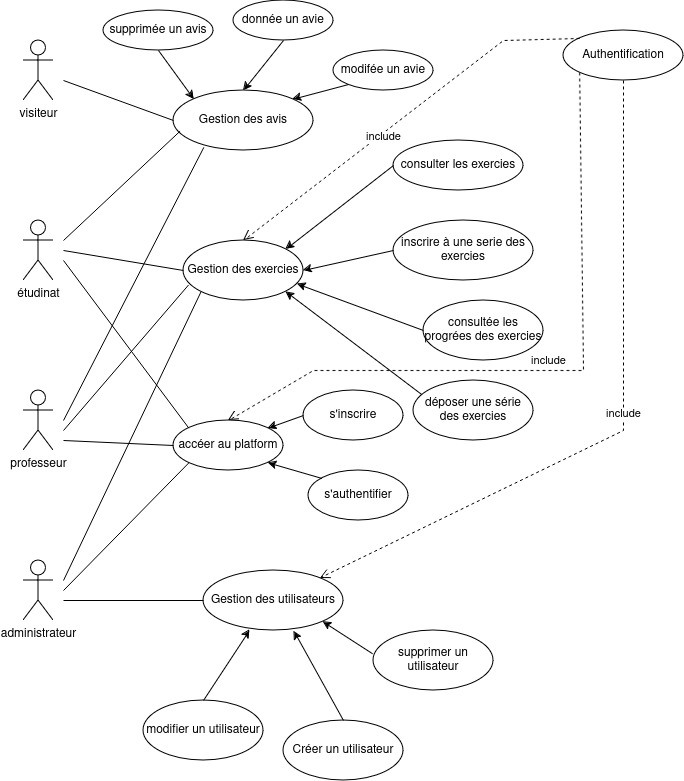
\includegraphics[width=0.6\textwidth]{pages/image/asma-usecase-global.jpg}
            \caption{pésentation de diagramme de cas d'utilisation}\label{fig:test}%
  \end{figure}

\section{Planification des sprints:}
 \subsection{\normal \series{ Sprint1: }Gestion d'accès de la plateforme}
Dans ce sprint, nous nous concentrerons sur la présentation de la manière dont nous avons réussi à mettre en place la gestion d'accès sur la plateforme en utilisant des techniques d'authentification. Nous énumérerons également les technologies utilisées pour créer une page de connexion et d'inscription adaptée et présentable. De plus, nous montrerons comment un utilisateur peut modifier certaines informations de son compte .
 
 \subsection {\normal \series{ Sprint2: }Gestion des exercises}
 Dans ce sprint, nous présenterons le processus de création d'une interface permettant aux utilisateurs d'accéder aux exercices fournis par le créateur des exercices (le professeur). Nous montrerons également comment compiler ces exercices en temps réel et stocker les résultats dans une base de données.
 
 \subsection {\normal \series{Sprint3: }Gestion des avis}
Ce sprint est principalement axé sur la fourniture aux utilisateurs de la possibilité de consulter la note des exercices en fonction des évaluations d'autres personnes à l'aide d'un système de notation. De plus, les utilisateurs pourront attribuer une note, la modifier et la supprimer après avoir terminer un exercice.

 \subsection {\normal \series{Sprint4: }Gestion des utilisateurs}
Ce chapitre se concentre sur la manière dont l'administrateur du site web interagit avec les utilisateurs et le contenu du site. L'administrateur a la capacité de manipuler (modification, supprission) des utilisateurs ou des exercices.















\section{Étude technologiques}
Dans cette partie, nous allons définir environnement matériel ainsi
que l’environnement logiciel afin d’élaborer ce projet.
\subsection{Environnement matériel}  
Cette plateforme a été développée avec un ordinateur Lenovo ayant les caractéristiques suivante:
\begin{itemize}
    \item  Processeur Dual Core AMD Athlon Silver 3050U   
      \item  Mémoire 12 Go
    \item Disque 512 Go SSD NV Me
    \item Carte graphique AMD Radeon Graphics Intégré 
\end{itemize}

\subsection{Environnement Logiciel}
 {\bf{ Visual Studio Code:}}
 Visual Studio Code est un éditeur de code open-source développé par Microsoft. Léger et puissant, il supporte de nombreux langages de programmation et offre des fonctionnalités telles que l'autocomplétion, le débogage et l'intégration Git. Avec ses extensions, VS Code s’adapte facilement aux besoins des développeurs.
 \begin{figure}[H]%
    \center%
    
\includegraphics[width=0.3\textwidth]{pages/images/vscode.png}
    \caption{ Logo Visual Studio Code}\label{fig:test}%
  \end{figure}

\vspace{10mm}
 {\bf{Postman :}}
 Postman est un outil populaire utilisé pour tester et interagir avec des APIs. Il permet de créer, envoyer et gérer des requêtes HTTP de manière simple et intuitive. Avec Postman, vous pouvez inspecter les réponses des APIs, automatiser les tests, et gérer des environnements de développement. C’est un outil essentiel pour les développeurs et les testeurs qui travaillent avec des services web et des interfaces de programmation.
 \begin{figure}[H]%
    \center%
    
\includegraphics[width=0.25\textwidth]{pages/images/postman.png}
    \caption{Logo Postman}\label{fig:test}%
  \end{figure}
 




{\bf{Mongo DataBase :}}
MongoDB est une base de données NoSQL orientée documents. Contrairement aux bases de données relationnelles, MongoDB stocke les données en format BSON (Binary JSON), ce qui permet une flexibilité accrue dans la gestion des données semi-structurées et non structurées. 
\\
Il est conçu pour évoluer horizontalement, facilitant ainsi la gestion de grandes quantités de données. MongoDB est apprécié pour sa performance, sa scalabilité et sa capacité à s'adapter aux besoins variés des applications modernes.
 \begin{figure}[H]%
    \center%
    
\includegraphics[width=0.3\textwidth]{pages/images/mongo.png}
    \caption{ Logo Mongo Data base}\label{fig:test}%
  \end{figure}





{\bf{Github :}}
GitHub est une plateforme de gestion de code source basée sur Git, qui facilite la collaboration entre développeurs.
\\
Elle permet de stocker et de suivre les versions du code, de gérer les projets avec des fonctionnalités telles que les demandes de tirage (pull requests), les issues, et les wikis.
\\
GitHub offre également des outils pour la collaboration en équipe, comme les revues de code et les intégrations continues, rendant le développement logiciel plus fluide et organisé.
 \begin{figure}[ht]%
    \center%
    
\includegraphics[width=0.25\textwidth]{pages/images/GitHub.png}
    \caption{ Logo Github}\label{fig:test}%
  \end{figure}







{\bf{Figma :}}
Figma est un outil de conception d'interface utilisateur et de prototypage collaboratif basé sur le cloud.
\\
Il permet aux designers de créer des maquettes interactives et des prototypes en temps réel tout en facilitant la collaboration entre les membres d'une équipe.
 Sa nature collaborative et ses fonctionnalités de versioning rendent le processus de conception plus fluide et intégré.
 \begin{figure}[H]%
    \center%
    
\includegraphics[width=0.3\textwidth]{pages/images/figma-1698087967030-2x.jpg}
    \caption{ Logo Figma }\label{fig:test}%
  \end{figure}





\subsection{Technologie et langage utilisée }
 {\bf{ ReactJS:}}
Est une bibliothèque JavaScript développée par Facebook pour la création d'interfaces utilisateur. Elle permet de construire des applications web dynamiques et réactives grâce à une approche basée sur des composants réutilisables. React utilise un DOM virtuel pour optimiser les mises à jour de l'interface, ce qui améliore les performances. Avec sa syntaxe JSX et son écosystème riche, ReactJS facilite le développement d'applications modernes et interactives.
 \begin{figure}[H]%
    \center%
    
\includegraphics[width=0.3\textwidth]{pages/images/react.png}
    \caption{ Logo ReactJS}\label{fig:test}%
  \end{figure}

 {\bf{ TypeScript:}}
Est un langage de programmation développé par Microsoft qui est une surcouche de JavaScript. Il ajoute des types statiques optionnels au langage, ce qui permet de détecter les erreurs de type lors de la compilation plutôt qu'à l'exécution. TypeScript offre également des fonctionnalités avancées comme les classes et les interfaces, facilitant ainsi le développement d'applications robustes et maintenables. Il se compile en JavaScript, ce qui permet une intégration facile avec les projets JavaScript existants.
 \begin{figure}[H]%
    \center%
    
\includegraphics[width=0.2\textwidth]{pages/images/typescript.png}
    \caption{ Logo TypeScript }\label{fig:test}%
  \end{figure}






 {\bf{ NodeJS:}}
 Est un environnement d'exécution JavaScript côté serveur, basé sur le moteur V8 de Google Chrome. 
\\
Il permet aux développeurs d'utiliser JavaScript pour écrire des scripts côté serveur, ce qui facilite le développement d'applications web évolutives et performantes. 
\\
Nodejs est réputé pour sa gestion efficace des opérations asynchrones et son architecture événementielle, ce qui le rend idéal pour les applications en temps réel comme les chats et les jeux en ligne. Avec un vaste écosystème de modules via npm, Node.js offre de nombreuses bibliothèques et outils pour enrichir vos projets.
 \begin{figure}[H]%
    \center%
    
\includegraphics[width=0.25\textwidth]{pages/images/nodejs.png}
    \caption{Logo NodeJS}\label{fig:test}%
  \end{figure}

 {\bf{ ExpressJS:}}
Express est un framework minimaliste pour Node.js, utilisé pour créer des applications web et des APIs.
\\
Il simplifie le processus de gestion des requêtes HTTP, la définition des routes, et le traitement des middleware.
\\
Express est apprécié pour sa flexibilité et sa simplicité, permettant aux développeurs de construire des applications robustes et performantes avec moins de configuration.
\\s
 \begin{figure}[H]%
    \center%
    
\includegraphics[width=0.2\textwidth]{pages/images/expressjs_logo_icon_169185.png}
    \caption{Logo Express JS}\label{fig:test}%
  \end{figure}







 {\bf{ tailwind CSS:}}
Est un framework de design utilitaire pour créer des interfaces web modernes et réactives.
Contrairement aux frameworks CSS traditionnels, Tailwind se base sur une approche de classes utilitaires qui permettent de styler directement les éléments HTML.
\\
Cette approche offre une grande flexibilité et un contrôle précis sur le design tout en évitant le besoin d'écrire des CSS personnalisés.
\begin{figure}[H]%
    \center%
    
\includegraphics[width=0.25\textwidth]{pages/images/tailwind.jpg}
    \caption{ Logo Tailwind CSS}\label{fig:test}%
  \end{figure}






\section{Justification des choix technologiques}
Le choix de React pour le front-end et Node.js pour le back-end s'appuie sur leur capacité à offrir des performances optimales, une modularité accrue, et une intégration fluide dans une plateforme éducative en ligne. React permet de créer des interfaces utilisateur dynamiques et réactives, avec une structure de composants réutilisables qui facilite le développement et la maintenance. Node.js, de son côté, assure une unification du langage JavaScript sur toute la stack, simplifiant la communication entre le front-end et le back-end et permettant de gérer efficacement un grand nombre de connexions simultanées, ce qui est essentiel pour une plateforme éducative évolutive et performante.






















\section { Conclusion}
\\
Dans ce chapitre, j’ai présenté le product Backlog et le diagramme global enfin j’ai présenté les logiciels et les langages utilisés dans le chapitre suivant, je vais présenter la première realisation.














